\documentclass[11pt]{article}
\usepackage[notes]{la}
\lamodule{6}{5}{Least-Squares Problems}
\laxdoc{1.4}
\laxdoc{1.5}
\laxdoc{1.7}
\laxdoc{2.1}
\laxdoc{2.3}
\laxdoc{6.1}
\laxdoc{6.2}
\laxdoc{6.3}
\laxdoc{6.4}

\begin{document}

\section{Least-Squares Problems}

\begin{guide}
In Chapter 1 a system $A\bv{x}=\bv{b}$ could end in a row $\begin{bmatrix}0&0&c\end{bmatrix}$ with $c\neq0$: no solution, because $\bv{b}$ is not in $\Col A$. Real data behave like this all the time. A table of measurements has more equations than unknowns, and the measurement errors make the system inconsistent. Saying ``no solution'' does not help. The useful question is: \emph{which $\bv{x}$ makes $A\bv{x}$ as close to $\bv{b}$ as possible?} Section 6.3 already answered the geometric half: the closest point of $\Col A$ to $\bv{b}$ is the projection $\proj_{\Col A}\bv{b}$ (the Best Approximation Theorem). This section turns that into an algorithm. The vector $\bv{x}$ we are after is a \emph{least-squares solution}, it satisfies the \emph{normal equations} $A\T A\bv{x}=A\T\bv{b}$, and when the columns of $A$ are independent we can also find it from a QR factorization. At the end we fit lines and curves to data.
\end{guide}

\textbf{By the end of this section you should be able to:}
\begin{itemize}
  \item explain what a least-squares solution of $A\bv{x}=\bv{b}$ is and why it exists;
  \item set up and solve the normal equations $A\T A\bv{x}=A\T\bv{b}$ by row reduction, and compute the least-squares error;
  \item decide when the least-squares solution is unique, and describe all of them when it is not;
  \item find a least-squares solution from a QR factorization by solving $R\bv{x}=Q\T\bv{b}$;
  \item fit a line, a line through the origin, or a polynomial to data by building a design matrix.
\end{itemize}

% ---------------------------------------------------------------------
\subsection*{When $A\bv{x}=\bv{b}$ has no solution}

\begin{exmp}{An inconsistent system}{noway}
Let $A=\begin{bmatrix}1&2\\1&0\\1&1\end{bmatrix}$ and $\bv{b}=(1,3,-1)$, so the system is $x_1+2x_2=1$, $x_1=3$, $x_1+x_2=-1$. Row reduce the augmented matrix:
\begin{align*}
\begin{amat}{cc|c}1 & 2 & 1\\1 & 0 & 3\\1 & 1 & -1\end{amat}
&\rops{R_2-R_1,R_3-R_1}
\begin{amat}{cc|c}1 & 2 & 1\\0 & -2 & 2\\0 & -1 & -2\end{amat}
\rops{-\tfrac12R_2}
\begin{amat}{cc|c}1 & 2 & 1\\0 & 1 & -1\\0 & -1 & -2\end{amat}
\rops{R_3+R_2}
\begin{amat}{cc|c}1 & 2 & 1\\0 & 1 & -1\\0 & 0 & -3\end{amat}
\end{align*}
The last row says $0x_1+0x_2=-3$. The system is inconsistent, which means that $\bv{b}$ is not a linear combination of the columns $\bv{a}_1=(1,1,1)$ and $\bv{a}_2=(2,0,1)$ (Theorem~\ref{1.4-thm:three}): $\bv{b}$ is not in $\Col A$.
\end{exmp}

No $\bv{x}$ makes $A\bv{x}-\bv{b}$ equal to $\bv{0}$. We settle for making it \emph{small}. For a candidate $\bv{x}$, the vector $\bv{b}-A\bv{x}$ is the \emph{residual}, and its length measures the failure.

\begin{defn}{Least-squares solution}{ls}
Let $A$ be an $m\times n$ matrix and $\bv{b}$ a vector in $\R^m$. A \emph{least-squares solution} of $A\bv{x}=\bv{b}$ is a vector $\hat{\bv{x}}$ in $\R^n$ such that
\[
\lVert\bv{b}-A\hat{\bv{x}}\rVert\le\lVert\bv{b}-A\bv{x}\rVert\qquad\text{for every }\bv{x}\text{ in }\R^n .
\]
\end{defn}

The name comes from $\lVert\bv{b}-A\bv{x}\rVert^2$, which is the sum of the \emph{squares} of the entries of the residual; making the length least makes this sum of squares least. If $A\bv{x}=\bv{b}$ has a solution, that solution makes the residual $\bv{0}$, so it is a least-squares solution (Example~\ref{ex:consist}).

\begin{exmp}{Three candidates}{compare}
Take $A$ and $\bv{b}$ of Example~\ref{ex:noway} and try three vectors $\bv{x}$. For $\bv{x}=(3,-1)$ we get $A\bv{x}=(1,3,2)$ and $\bv{b}-A\bv{x}=(0,0,-3)$, of squared length $9$. For $\bv{x}=(1,0)$ we get $A\bv{x}=(1,1,1)$ and $\bv{b}-A\bv{x}=(0,2,-2)$, of squared length $8$. For $\bv{x}=(2,-1)$ we get $A\bv{x}=(0,2,1)$ and $\bv{b}-A\bv{x}=(1,1,-2)$, of squared length $6$. The first candidate solves two of the three equations exactly and still does worst. Is $(2,-1)$ the best of all $\bv{x}$ in $\R^2$, or only the best of the three? Section 6.3 will decide it.
\end{exmp}

% ---------------------------------------------------------------------
\subsection*{The normal equations}

For every $\bv{x}$ the vector $A\bv{x}$ lies in $\Col A$, and as $\bv{x}$ runs through $\R^n$ it runs through all of $\Col A$. So minimizing $\lVert\bv{b}-A\bv{x}\rVert$ is exactly the problem ``find the point of $\Col A$ closest to $\bv{b}$'', and that point is $\hat{\bv{b}}=\proj_{\Col A}\bv{b}$.

\begin{thm}{The normal equations}{normal}
Let $A$ be an $m\times n$ matrix, let $\bv{b}$ be in $\R^m$ and let $\hat{\bv{b}}=\proj_{\Col A}\bv{b}$.
\begin{enumerate}[label=(\alph*),itemsep=1pt]
  \item A least-squares solution of $A\bv{x}=\bv{b}$ exists. A vector $\hat{\bv{x}}$ is one if and only if $A\hat{\bv{x}}=\hat{\bv{b}}$.
  \item A vector $\hat{\bv{x}}$ is a least-squares solution if and only if it solves the \emph{normal equations}
  \[
  A\T A\,\bv{x}=A\T\bv{b}.
  \]
\end{enumerate}
\end{thm}

\begin{proof}
The column space is spanned by the columns of $A$, so by Theorem~\ref{6.4-thm:exist} the projection $\hat{\bv{b}}$ exists, and by Theorem~\ref{6.3-thm:best} it is the \emph{only} point of $\Col A$ at the least distance from $\bv{b}$: every other point $\bv{v}$ of $\Col A$ has $\lVert\bv{b}-\hat{\bv{b}}\rVert<\lVert\bv{b}-\bv{v}\rVert$.

(a)~Since $\hat{\bv{b}}$ is in $\Col A$, there is an $\hat{\bv{x}}$ with $A\hat{\bv{x}}=\hat{\bv{b}}$; this proves existence once we know such an $\hat{\bv{x}}$ is least-squares. If $A\hat{\bv{x}}=\hat{\bv{b}}$, then for every $\bv{x}$ the point $A\bv{x}$ of $\Col A$ is at least as far from $\bv{b}$ as $\hat{\bv{b}}$, so $\lVert\bv{b}-A\hat{\bv{x}}\rVert\le\lVert\bv{b}-A\bv{x}\rVert$. Conversely, let $\hat{\bv{x}}$ be least-squares. Choose $\bv{x}_0$ with $A\bv{x}_0=\hat{\bv{b}}$. Then $\lVert\bv{b}-A\hat{\bv{x}}\rVert\le\lVert\bv{b}-A\bv{x}_0\rVert=\lVert\bv{b}-\hat{\bv{b}}\rVert$. If $A\hat{\bv{x}}$ were different from $\hat{\bv{b}}$, the strict inequality above would give $\lVert\bv{b}-\hat{\bv{b}}\rVert<\lVert\bv{b}-A\hat{\bv{x}}\rVert$, a contradiction. So $A\hat{\bv{x}}=\hat{\bv{b}}$.

(b)~Suppose $A\hat{\bv{x}}=\hat{\bv{b}}$. Then $\bv{b}-A\hat{\bv{x}}=\bv{b}-\hat{\bv{b}}$ is in $(\Col A)^{\perp}$, so it is orthogonal to every column $\bv{a}_j$ of $A$. The entries of $A\T(\bv{b}-A\hat{\bv{x}})$ are exactly the numbers $\bv{a}_j\cdot(\bv{b}-A\hat{\bv{x}})$ (Theorem~\ref{1.4-thm:rowcol}, because the rows of $A\T$ are the columns of $A$), so $A\T(\bv{b}-A\hat{\bv{x}})=\bv{0}$, that is $A\T A\hat{\bv{x}}=A\T\bv{b}$.

Conversely, suppose $A\T A\hat{\bv{x}}=A\T\bv{b}$. Then $A\T(\bv{b}-A\hat{\bv{x}})=\bv{0}$, so $\bv{b}-A\hat{\bv{x}}$ is orthogonal to every column of $A$ and therefore lies in $(\Col A)^{\perp}$ (Theorem~\ref{6.1-thm:perpfacts}(a)). Now $\bv{b}=A\hat{\bv{x}}+(\bv{b}-A\hat{\bv{x}})$ splits $\bv{b}$ into a vector of $\Col A$ and a vector of $(\Col A)^{\perp}$. By the uniqueness in Theorem~\ref{6.3-thm:decomp}(a) this split is $\hat{\bv{b}}+(\bv{b}-\hat{\bv{b}})$, so $A\hat{\bv{x}}=\hat{\bv{b}}$, and $\hat{\bv{x}}$ is least-squares by part~(a).
\end{proof}

\begin{proc}{Least squares by the normal equations}{normproc}
Given $A$ ($m\times n$) and $\bv{b}$:
\begin{enumerate}[nosep]
  \item compute the $n\times n$ matrix $A\T A$ and the vector $A\T\bv{b}$ (their entries are dot products of the columns of $A$ with each other and with $\bv{b}$);
  \item row reduce the augmented matrix $\begin{bmatrix}A\T A&A\T\bv{b}\end{bmatrix}$; by Theorem~\ref{thm:normal} it is consistent;
  \item read off $\hat{\bv{x}}$ (with free variables if there are any, Theorem~\ref{thm:uniq});
  \item check: $\hat{\bv{b}}=A\hat{\bv{x}}$, the residual $\bv{b}-\hat{\bv{b}}$ is orthogonal to the columns of $A$, and compute its length.
\end{enumerate}
\end{proc}

\begin{exmp}{Solving the normal equations}{normex}
Return to $A$ and $\bv{b}$ of Example~\ref{ex:noway}, with $\bv{a}_1=(1,1,1)$, $\bv{a}_2=(2,0,1)$. The entries of $A\T A$ are $\bv{a}_1\cdot\bv{a}_1=3$, $\bv{a}_1\cdot\bv{a}_2=3$, $\bv{a}_2\cdot\bv{a}_2=5$, and $A\T\bv{b}=(\bv{a}_1\cdot\bv{b},\bv{a}_2\cdot\bv{b})=(1+3-1,\ 2+0-1)=(3,1)$. Row reduce the augmented matrix:
\begin{align*}
\begin{amat}{cc|c}3 & 3 & 3\\3 & 5 & 1\end{amat}
&\rops{R_2-R_1}
\begin{amat}{cc|c}3 & 3 & 3\\0 & 2 & -2\end{amat}
\rops{\tfrac13R_1,\tfrac12R_2}
\begin{amat}{cc|c}1 & 1 & 1\\0 & 1 & -1\end{amat}
\rops{R_1-R_2}
\begin{amat}{cc|c}1 & 0 & 2\\0 & 1 & -1\end{amat}
\end{align*}
So $\hat{\bv{x}}=(2,-1)$, the vector that came out best in Example~\ref{ex:compare}, and now we know it is best among \emph{all} vectors. Then $\hat{\bv{b}}=A\hat{\bv{x}}=2(1,1,1)-(2,0,1)=(0,2,1)$ and the residual is $\bv{b}-\hat{\bv{b}}=(1,3,-1)-(0,2,1)=(1,1,-2)$. Check: $\bv{a}_1\cdot(1,1,-2)=1+1-2=0$ and $\bv{a}_2\cdot(1,1,-2)=2+0-2=0$. \ $\checkmark$ The least-squares error is $\lVert(1,1,-2)\rVert=\sqrt6$.
\end{exmp}

\begin{center}
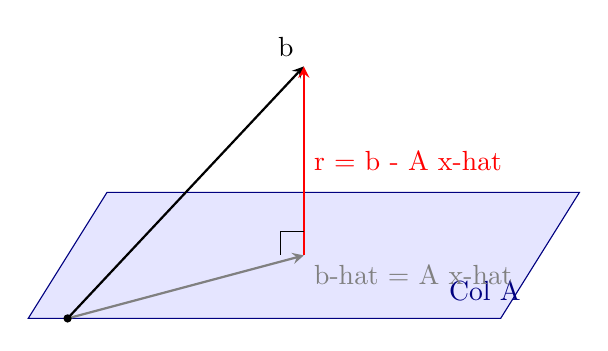
\begin{tikzpicture}[>=stealth,scale=1.0]
  \fill[blue!10] (-0.5,0)--(5.5,0)--(6.5,1.6)--(0.5,1.6)--cycle;
  \draw[blue!50!black] (-0.5,0)--(5.5,0)--(6.5,1.6)--(0.5,1.6)--cycle;
  \node[blue!50!black] at (5.3,0.35) {Col A};
  \draw[->,thick] (0,0)--(3,3.2) node[above left] {b};
  \draw[->,thick,gray] (0,0)--(3,0.8) node[below right] {b-hat = A x-hat};
  \draw[->,thick,red] (3,0.8)--(3,3.2) node[midway,right] {r = b - A x-hat};
  \draw (3,1.1)--(2.7,1.1)--(2.7,0.8);
  \fill (0,0) circle (1.5pt);
\end{tikzpicture}
\end{center}

\noindent\textbf{Figure 1.} The plane stands for $\Col A$. The point $A\hat{\bv{x}}=\hat{\bv{b}}$ is the foot of the perpendicular from $\bv{b}$ to the plane, and the residual $\bv{r}=\bv{b}-A\hat{\bv{x}}$ is perpendicular to every vector of the plane. This picture is Figure~2 of Section 6.3 with a name for the weights $\hat{\bv{x}}$.

\begin{warn}[x-hat does not solve the original system]
The vector $\hat{\bv{x}}$ solves $A\T A\bv{x}=A\T\bv{b}$, not $A\bv{x}=\bv{b}$. In Example~\ref{ex:normex}, $A\hat{\bv{x}}=(0,2,1)$ is not $\bv{b}=(1,3,-1)$. Every solution of $A\bv{x}=\bv{b}$ also solves the normal equations (multiply both sides by $A\T$), but the reverse is false.
\end{warn}

\begin{defn}{Least-squares error}{err}
The \emph{least-squares error} of $A\bv{x}=\bv{b}$ is $\lVert\bv{b}-A\hat{\bv{x}}\rVert$ for a least-squares solution $\hat{\bv{x}}$. By Theorem~\ref{thm:normal}(a) it equals $\lVert\bv{b}-\hat{\bv{b}}\rVert$, the distance from $\bv{b}$ to $\Col A$ (Definition~\ref{6.3-def:dist}), so it does not depend on which least-squares solution is used.
\end{defn}

Because $\hat{\bv{b}}$ is in $\Col A$ and the residual is in $(\Col A)^{\perp}$, they are orthogonal, and the Pythagorean theorem (Theorem~\ref{6.1-thm:pyth}) gives $\lVert\bv{b}\rVert^2=\lVert\hat{\bv{b}}\rVert^2+\lVert\bv{b}-\hat{\bv{b}}\rVert^2$. In Example~\ref{ex:normex}: $\lVert\bv{b}\rVert^2=1+9+1=11$, $\lVert\hat{\bv{b}}\rVert^2=0+4+1=5$ and the squared error is $6$. \ $\checkmark$

\begin{exmp}{A consistent system}{consist}
With the same $A$ take $\bv{b}=(5,3,4)$. Now $A\T\bv{b}=(5+3+4,\ 10+0+4)=(12,14)$ and
\begin{align*}
\begin{amat}{cc|c}3 & 3 & 12\\3 & 5 & 14\end{amat}
&\rops{R_2-R_1}
\begin{amat}{cc|c}3 & 3 & 12\\0 & 2 & 2\end{amat}
\rops{\tfrac13R_1,\tfrac12R_2}
\begin{amat}{cc|c}1 & 1 & 4\\0 & 1 & 1\end{amat}
\rops{R_1-R_2}
\begin{amat}{cc|c}1 & 0 & 3\\0 & 1 & 1\end{amat}
\end{align*}
gives $\hat{\bv{x}}=(3,1)$, and $A\hat{\bv{x}}=3(1,1,1)+(2,0,1)=(5,3,4)=\bv{b}$. The residual is $\bv{0}$ and the error is $0$: when the system is consistent its solutions are exactly its least-squares solutions (this is proved in Example~\ref{ex:b-consis}).
\end{exmp}

\begin{exmp}{The entries of $A\T A$ are dot products}{gram}
For $A=\begin{bmatrix}1&2\\1&0\\1&1\end{bmatrix}$ the entry in row $i$ and column $j$ of $A\T A$ is $\bv{a}_i\cdot\bv{a}_j$, because row $i$ of $A\T$ is column $i$ of $A$. So $A\T A$ is $2\times2$ although $A$ is $3\times2$, and it is symmetric, since $\bv{a}_i\cdot\bv{a}_j=\bv{a}_j\cdot\bv{a}_i$. In general $A\T A$ is always an $n\times n$ matrix when $A$ is $m\times n$, which is why the normal equations always have as many equations as unknowns.
\end{exmp}

\begin{think}{One point, many weights?}{closest}
Theorem~\ref{thm:normal} says every least-squares solution $\hat{\bv{x}}$ satisfies $A\hat{\bv{x}}=\hat{\bv{b}}$. Could two different least-squares solutions give two different vectors $A\hat{\bv{x}}$? What does that say about the least-squares error?
\end{think}

\begin{kc}{Set up and solve}{kcnormal}
Let $A=\begin{bmatrix}1&1\\1&0\\0&1\end{bmatrix}$ and $\bv{b}=(1,2,2)$. Write down $A\T A$ and $A\T\bv{b}$, solve the normal equations, and find the residual. Check that it is orthogonal to both columns.
\end{kc}

\begin{kc}{Is this the best $\bv{x}$?}{kctest}
For $A$ and $\bv{b}$ of Example~\ref{ex:noway}, is $\bv{x}=(3,-1)$ a least-squares solution? Decide by computing $A\T(\bv{b}-A\bv{x})$; do not solve the normal equations.
\end{kc}

% ---------------------------------------------------------------------
\subsection*{Uniqueness, and what to do when it fails}

Is the answer $\hat{\bv{x}}$ the only one? The vector $\hat{\bv{b}}$ is unique, but several $\bv{x}$ can be sent to it, exactly as in Chapter 1 where a consistent system has many solutions when there are free variables.

\begin{thm}{Uniqueness of the least-squares solution}{uniq}
Let $A$ be an $m\times n$ matrix.
\begin{enumerate}[label=(\alph*),itemsep=1pt]
  \item $A\T A\bv{x}=\bv{0}$ if and only if $A\bv{x}=\bv{0}$.
  \item If $\hat{\bv{x}}_p$ is one least-squares solution of $A\bv{x}=\bv{b}$, the set of all of them is $\{\hat{\bv{x}}_p+\bv{w}:\ A\bv{w}=\bv{0}\}$.
  \item The following are equivalent: (i)~the least-squares solution is unique for every $\bv{b}$ (equivalently, for one $\bv{b}$); (ii)~the columns of $A$ are linearly independent; (iii)~the $n\times n$ matrix $A\T A$ is invertible. In that case $\hat{\bv{x}}=(A\T A)^{-1}A\T\bv{b}$.
\end{enumerate}
\end{thm}

\begin{proof}
(a)~If $A\bv{x}=\bv{0}$ then $A\T A\bv{x}=A\T\bv{0}=\bv{0}$. Conversely, suppose $A\T A\bv{x}=\bv{0}$. Multiply by $\bv{x}\T$: $0=\bv{x}\T A\T A\bv{x}=(A\bv{x})\T(A\bv{x})=\lVert A\bv{x}\rVert^2$, using $(A\bv{x})\T=\bv{x}\T A\T$ (Theorem~\ref{2.1-thm:transprops}(d)). A vector of length $0$ is $\bv{0}$ (Theorem~\ref{6.1-thm:dotprops}(d)), so $A\bv{x}=\bv{0}$.

(b)~By Theorem~\ref{thm:normal}(a) the least-squares solutions are exactly the solutions of $A\bv{x}=\hat{\bv{b}}$. This system is consistent and $\hat{\bv{x}}_p$ is one solution, so by Theorem~\ref{1.5-thm:translate} the solution set is $\hat{\bv{x}}_p+\{\bv{w}:A\bv{w}=\bv{0}\}$.

(c)~By (b) the least-squares solution is unique exactly when $A\bv{w}=\bv{0}$ has only the trivial solution, that is, when the columns of $A$ are independent (Theorem~\ref{1.7-thm:cols}); this is (i)$\Leftrightarrow$(ii), and the answer does not depend on $\bv{b}$. By (a), $A\T A\bv{x}=\bv{0}$ has only the trivial solution if and only if $A\bv{x}=\bv{0}$ does, so the square matrix $A\T A$ satisfies statement (d) of the Invertible Matrix Theorem (Theorem~\ref{2.3-thm:imt}) exactly when the columns of $A$ are independent; this is (ii)$\Leftrightarrow$(iii). Finally, if $A\T A$ is invertible, multiplying the normal equations by $(A\T A)^{-1}$ gives $\hat{\bv{x}}=(A\T A)^{-1}A\T\bv{b}$.
\end{proof}

\begin{exmp}{Dependent columns}{dep}
Add to the matrix of Example~\ref{ex:noway} a third column $\bv{a}_3=\bv{a}_1+\bv{a}_2=(3,1,2)$, and keep $\bv{b}=(1,3,-1)$:
\[
A=\begin{bmatrix}1&2&3\\1&0&1\\1&1&2\end{bmatrix}.
\]
The dot products give $A\T A=\begin{bmatrix}3&3&6\\3&5&8\\6&8&14\end{bmatrix}$ and $A\T\bv{b}=(3,\ 1,\ 3+3-2)=(3,1,4)$. Row reduce:
\begin{align*}
\begin{amat}{ccc|c}3 & 3 & 6 & 3\\3 & 5 & 8 & 1\\6 & 8 & 14 & 4\end{amat}
&\rops{R_2-R_1,R_3-2R_1}
\begin{amat}{ccc|c}3 & 3 & 6 & 3\\0 & 2 & 2 & -2\\0 & 2 & 2 & -2\end{amat}
\rops{R_3-R_2}
\begin{amat}{ccc|c}3 & 3 & 6 & 3\\0 & 2 & 2 & -2\\0 & 0 & 0 & 0\end{amat}\\
&\rops{\tfrac13R_1,\tfrac12R_2}
\begin{amat}{ccc|c}1 & 1 & 2 & 1\\0 & 1 & 1 & -1\\0 & 0 & 0 & 0\end{amat}
\rops{R_1-R_2}
\begin{amat}{ccc|c}1 & 0 & 1 & 2\\0 & 1 & 1 & -1\\0 & 0 & 0 & 0\end{amat}
\end{align*}
The variable $x_3$ is free: $\hat{\bv{x}}=(2,-1,0)+x_3(-1,-1,1)$. The vector $(-1,-1,1)$ solves $A\bv{w}=\bv{0}$, because $-\bv{a}_1-\bv{a}_2+\bv{a}_3=\bv{0}$, as Theorem~\ref{thm:uniq}(b) says. Two members of the family: $x_3=0$ gives $(2,-1,0)$ and $A(2,-1,0)=2\bv{a}_1-\bv{a}_2=(0,2,1)$; $x_3=1$ gives $(1,-2,1)$ and $A(1,-2,1)=\bv{a}_1-2\bv{a}_2+\bv{a}_3=(0,2,1)$. Both give the same $\hat{\bv{b}}=(0,2,1)$ as in Example~\ref{ex:normex}, since the new column adds nothing to $\Col A$.
\end{exmp}

\begin{think}{Why a free variable is not a failure}{freevar}
In Example~\ref{ex:dep} the normal equations have a free variable, yet the least-squares error is the same $\sqrt6$ as in Example~\ref{ex:normex}. Why does non-uniqueness of $\hat{\bv{x}}$ not affect the error?
\end{think}

\begin{kc}{Unique or not?}{kcuniq}
Let $A=\begin{bmatrix}1&2\\2&4\\3&6\end{bmatrix}$. Is the least-squares solution of $A\bv{x}=\bv{b}$ unique for every $\bv{b}$? How many least-squares solutions are there for $\bv{b}=(1,0,0)$?
\end{kc}

% ---------------------------------------------------------------------
\subsection*{Least squares from a QR factorization}

The normal equations square the columns of $A$ and then ask for a row reduction. When the columns are independent, Section 6.4 offers a way around: write $A=QR$ and let $Q$ do the projecting.

\begin{thm}{Least squares by QR}{qrls}
Let $A$ be an $m\times n$ matrix with linearly independent columns and let $A=QR$ be a QR factorization (Definition~\ref{6.4-def:qr}). Then for every $\bv{b}$ in $\R^m$ the equation $A\bv{x}=\bv{b}$ has exactly one least-squares solution $\hat{\bv{x}}$, namely the solution of
\[
R\bv{x}=Q\T\bv{b},\qquad\text{that is}\qquad\hat{\bv{x}}=R^{-1}Q\T\bv{b},
\]
and $\hat{\bv{b}}=QQ\T\bv{b}$.
\end{thm}

\begin{proof}
By Theorem~\ref{6.4-thm:qrthm} the columns of $Q$ are an orthonormal basis of $\Col A$, so Theorem~\ref{6.3-thm:orthonormal} gives $\hat{\bv{b}}=\proj_{\Col A}\bv{b}=QQ\T\bv{b}$. By Theorem~\ref{thm:normal}(a), $\hat{\bv{x}}$ is a least-squares solution if and only if $A\hat{\bv{x}}=\hat{\bv{b}}$, that is, $QR\hat{\bv{x}}=QQ\T\bv{b}$.

If $\hat{\bv{x}}$ satisfies this, multiply on the left by $Q\T$ and use $Q\T Q=I$ (Theorem~\ref{6.2-thm:utu}): $R\hat{\bv{x}}=Q\T\bv{b}$. Conversely, if $R\hat{\bv{x}}=Q\T\bv{b}$, multiply on the left by $Q$: $QR\hat{\bv{x}}=QQ\T\bv{b}$.

The matrix $R$ is triangular with positive diagonal entries, so it is invertible (Theorem~\ref{2.3-thm:triangular}), and $R\bv{x}=Q\T\bv{b}$ has exactly one solution, found by back-substitution.
\end{proof}

\begin{proc}{Least squares by QR}{qrproc}
Given $A$ with independent columns and $\bv{b}$:
\begin{enumerate}[nosep]
  \item find $A=QR$ (Procedure~\ref{6.4-proc:qrproc});
  \item compute $Q\T\bv{b}$;
  \item solve the triangular system $R\bv{x}=Q\T\bv{b}$ by back-substitution;
  \item check: $\hat{\bv{b}}=A\hat{\bv{x}}$, and the squared error is $\lVert\bv{b}\rVert^2-\lVert Q\T\bv{b}\rVert^2$ (Pause and think~\ref{think:qrerr}).
\end{enumerate}
\end{proc}

\begin{exmp}{Solving by QR and by the normal equations}{qrex}
Let $A=\begin{bmatrix}1&4\\2&5\\2&2\end{bmatrix}$ and $\bv{b}=(7,5,5)$. Gram--Schmidt on the columns $\bv{x}_1=(1,2,2)$, $\bv{x}_2=(4,5,2)$: $\bv{v}_1=\bv{x}_1$ with $\bv{v}_1\cdot\bv{v}_1=9$; $\bv{x}_2\cdot\bv{v}_1=4+10+4=18$, so $\bv{v}_2=\bv{x}_2-2\bv{v}_1=(2,1,-2)$. Both have length $3$, hence
\[
Q=\tfrac13\begin{bmatrix}1&2\\2&1\\2&-2\end{bmatrix},\qquad R=Q\T A=\tfrac13\begin{bmatrix}1&2&2\\2&1&-2\end{bmatrix}\begin{bmatrix}1&4\\2&5\\2&2\end{bmatrix}=\tfrac13\begin{bmatrix}9&18\\0&9\end{bmatrix}=\begin{bmatrix}3&6\\0&3\end{bmatrix}.
\]
Now $Q\T\bv{b}=\tfrac13(7+10+10,\ 14+5-10)=(9,3)$, and $R\bv{x}=(9,3)$ reads $3x_1+6x_2=9$, $3x_2=3$. Back-substitution gives $x_2=1$ and $3x_1=9-6$, so $\hat{\bv{x}}=(1,1)$. Then $\hat{\bv{b}}=A\hat{\bv{x}}=(5,7,4)$ and the residual is $(2,-2,1)$. Check: $(1,2,2)\cdot(2,-2,1)=2-4+2=0$ and $(4,5,2)\cdot(2,-2,1)=8-10+2=0$. \ $\checkmark$ The error is $\sqrt{4+4+1}=3$, and indeed $\lVert\bv{b}\rVert^2-\lVert Q\T\bv{b}\rVert^2=99-(81+9)=9$.

\emph{The normal equations for the same problem.} $A\T A=\begin{bmatrix}9&18\\18&45\end{bmatrix}$ and $A\T\bv{b}=(7+10+10,\ 28+25+10)=(27,63)$. Subtracting twice the first equation $9x_1+18x_2=27$ from the second leaves $9x_2=9$, so $x_2=1$ and $x_1=1$. Same answer, with larger numbers.
\end{exmp}

\begin{warn}[Q-transpose and not Q-inverse]
The solution is $R^{-1}Q\T\bv{b}$, not $R^{-1}Q^{-1}\bv{b}$. The matrix $Q$ is $m\times n$ and has no inverse when $m>n$; what it has is $Q\T Q=I_n$. Also note that $QQ\T\neq I_m$ in that case: $QQ\T\bv{b}$ is the projection $\hat{\bv{b}}$, not $\bv{b}$.
\end{warn}

Software uses QR rather than the normal equations because forming $A\T A$ magnifies rounding errors; we state this without proof. For hand work, both are fine, and the choice is mostly taste: the normal equations need no Gram--Schmidt, QR needs no row reduction.

\begin{think}{The error from $Q\T\bv{b}$}{qrerr}
Why is $\lVert\bv{b}-\hat{\bv{b}}\rVert^2=\lVert\bv{b}\rVert^2-\lVert Q\T\bv{b}\rVert^2$ when $\hat{\bv{b}}=QQ\T\bv{b}$? Use Theorem~\ref{6.2-thm:preserve} and the Pythagorean theorem.
\end{think}

\begin{kc}{Use the factorization}{kcqr}
Use $Q$ and $R$ of Example~\ref{ex:qrex} to find the least-squares solution of $A\bv{x}=\bv{b}$ for $\bv{b}=(5,1,1)$, and its error.
\end{kc}

% ---------------------------------------------------------------------
\subsection*{Fitting a line, or a curve, to data}

The main use of least squares is to fit a formula to measurements. Suppose measurements give points $(t_1,y_1),\dots,(t_m,y_m)$ and we want a model $y=c_0+c_1t$. If all points were on one line, then $c_0+c_1t_i=y_i$ for each $i$, which is the system
\[
\begin{bmatrix}1&t_1\\1&t_2\\\vdots&\vdots\\1&t_m\end{bmatrix}\begin{bmatrix}c_0\\c_1\end{bmatrix}=\begin{bmatrix}y_1\\y_2\\\vdots\\y_m\end{bmatrix}.
\]
It is almost never consistent, and a least-squares solution gives the line that makes the sum of the squares of the vertical gaps $y_i-(c_0+c_1t_i)$ least.

\begin{defn}{Design matrix and linear model}{design}
Let $f_0,f_1,\dots,f_d$ be given functions. The model $y=c_0f_0(t)+c_1f_1(t)+\cdots+c_df_d(t)$ and the data $(t_1,y_1),\dots,(t_m,y_m)$ lead to the system $X\bv{c}=\bv{y}$, where $\bv{y}=(y_1,\dots,y_m)$, $\bv{c}=(c_0,\dots,c_d)$ and the \emph{design matrix} $X$ has the entries $X_{ij}=f_j(t_i)$. A least-squares solution $\hat{\bv{c}}$ of $X\bv{c}=\bv{y}$ gives the \emph{best-fit} model. The \emph{residual vector} is $\bv{r}=\bv{y}-X\hat{\bv{c}}$.
\end{defn}

The model is called \emph{linear} because it is linear in the unknowns $c_0,\dots,c_d$; the functions $f_j$ may be as curved as we like. The next theorem says when the best fit is unique. For polynomials, $f_j(t)=t^j$ and the columns of $X$ are $(1,\dots,1)$, $(t_1,\dots,t_m)$, $(t_1^2,\dots,t_m^2)$ and so on.

\begin{thm}{Polynomial fits}{poly}
Fit a polynomial $y=c_0+c_1t+\cdots+c_dt^d$ to data with $t$-values $t_1,\dots,t_m$. The columns of the design matrix are linearly independent if and only if at least $d+1$ of the numbers $t_1,\dots,t_m$ are different. In that case the best-fit polynomial is unique and $\hat{\bv{c}}=(X\T X)^{-1}X\T\bv{y}$.
\end{thm}

\begin{proof}
The columns of $X$ are dependent if and only if $X\bv{c}=\bv{0}$ for some $\bv{c}\neq\bv{0}$. The $i$th entry of $X\bv{c}$ is $p(t_i)$ where $p(t)=c_0+c_1t+\cdots+c_dt^d$, and $\bv{c}\neq\bv{0}$ means that $p$ is not the zero polynomial. So the columns are dependent if and only if some nonzero polynomial of degree at most $d$ vanishes at every $t_i$.

We use one fact from algebra, which we do not prove here: a nonzero polynomial of degree at most $d$ has at most $d$ different roots. If at least $d+1$ of the $t_i$ are different, no such $p$ exists, so the columns are independent. If at most $d$ different values $s_1,\dots,s_k$ occur among the $t_i$ (so $k\le d$), the polynomial $p(t)=(t-s_1)\cdots(t-s_k)$ is nonzero, has degree $k\le d$, and vanishes at every $t_i$; so the columns are dependent.

The last sentence is Theorem~\ref{thm:uniq}(c) applied to $X$.
\end{proof}

For a line ($d=1$) the entries of $X\T X$ and $X\T\bv{y}$ are dot products of the columns $(1,\dots,1)$ and $(t_1,\dots,t_m)$ with each other and with $\bv{y}$:
\[
X\T X=\begin{bmatrix}m&\sum t_i\\\sum t_i&\sum t_i^2\end{bmatrix},\qquad X\T\bv{y}=\begin{bmatrix}\sum y_i\\\sum t_iy_i\end{bmatrix}.
\]

\begin{proc}{Fitting a model to data}{fitproc}
\begin{enumerate}[nosep]
  \item Choose the model, that is, the functions $f_0,\dots,f_d$.
  \item Build the design matrix $X$ (one row per data point) and the vector $\bv{y}$.
  \item Solve the normal equations $X\T X\bv{c}=X\T\bv{y}$ (or use a QR factorization of $X$).
  \item Write the fitted function, compute the fitted values $X\hat{\bv{c}}$ and the residual $\bv{r}=\bv{y}-X\hat{\bv{c}}$, and check that $X\T\bv{r}=\bv{0}$.
\end{enumerate}
\end{proc}

\begin{exmp}{A line through four points}{linefit}
A seedling is measured once a week: its height is $2,3,5,6$ cm at weeks $t=0,1,2,3$. The design matrix and the data vector are
\[
X=\begin{bmatrix}1&0\\1&1\\1&2\\1&3\end{bmatrix},\qquad\bv{y}=(2,3,5,6).
\]
The entries are $m=4$, $\sum t_i=0+1+2+3=6$, $\sum t_i^2=0+1+4+9=14$, $\sum y_i=2+3+5+6=16$ and $\sum t_iy_i=0+3+10+18=31$. Row reduce $\begin{bmatrix}X\T X&X\T\bv{y}\end{bmatrix}$:
\begin{align*}
\begin{amat}{cc|c}4 & 6 & 16\\6 & 14 & 31\end{amat}
&\rops{R_2-\tfrac32R_1}
\begin{amat}{cc|c}4 & 6 & 16\\0 & 5 & 7\end{amat}
\rops{\tfrac14R_1,\tfrac15R_2}
\begin{amat}{cc|c}1 & \tfrac32 & 4\\0 & 1 & \tfrac75\end{amat}
\rops{R_1-\tfrac32R_2}
\begin{amat}{cc|c}1 & 0 & \tfrac{19}{10}\\0 & 1 & \tfrac75\end{amat}
\end{align*}
The best-fit line is $y=\tfrac{19}{10}+\tfrac75\,t$. The fitted values are $X\hat{\bv{c}}=\tfrac1{10}(19,33,47,61)$ and the residual vector is $\bv{r}=\bv{y}-X\hat{\bv{c}}=\tfrac1{10}(1,-3,3,-1)$. Check: $\sum r_i=\tfrac1{10}(1-3+3-1)=0$ and $\sum t_ir_i=\tfrac1{10}(0-3+6-3)=0$, so $X\T\bv{r}=\bv{0}$. \ $\checkmark$ The squared error is $\tfrac1{100}(1+9+9+1)=\tfrac15$. The line predicts a height of $\tfrac{19}{10}+7=8.9$ cm at week $5$; a prediction outside the weeks that were measured is only as good as the assumption that growth stays linear.
\end{exmp}

\begin{center}
\begin{tikzpicture}[>=stealth,scale=1.0]
  \draw[->] (0,0)--(4.6,0) node[right] {t (weeks)};
  \draw[->] (0,0)--(0,3.6) node[above] {y (cm)};
  \draw[thick,blue!60!black] (0,0.95)--(3.4,3.33);
  \foreach \x/\y in {0/1,1/1.5,2/2.5,3/3} {\fill[red!70!black] (\x,\y) circle (2.5pt);}
  \draw[gray] (0,0.95)--(0,1);
  \draw[gray] (1,1.65)--(1,1.5);
  \draw[gray] (2,2.35)--(2,2.5);
  \draw[gray] (3,3.05)--(3,3);
  \node at (3.9,2.6) {y = 1.9 + 1.4 t};
\end{tikzpicture}
\end{center}

\noindent\textbf{Figure 2.} The four measurements of Example~\ref{ex:linefit} (the heights are drawn at half scale) and the best-fit line. The residuals are the vertical gaps between each point and the line.

\begin{exmp}{Two data points}{twopoints}
Fit a line to the two points $(1,4)$ and $(3,10)$. Here $d=1$ and there are two different $t$-values, so by Theorem~\ref{thm:poly} the fit is unique. The system $c_0+c_1=4$, $c_0+3c_1=10$ is consistent: $c_1=3$ and $c_0=1$. By Example~\ref{ex:consist} the least-squares solution is this exact solution, and the error is $0$: a line fitted to two points passes through both.
\end{exmp}

\begin{exmp}{Two measurements at the same time}{samet}
Fit a line to $(1,2)$ and $(1,4)$. Now the two $t$-values coincide, so there are fewer than $d+1=2$ different ones, and Theorem~\ref{thm:poly} says the best fit is not unique. Here $X=\begin{bmatrix}1&1\\1&1\end{bmatrix}$, $\bv{y}=(2,4)$, the columns are equal, and every $(c_0,c_1)$ with $c_0+c_1=3$ gives the same fitted values $(3,3)$ and residual $(-1,1)$. Every line through $(1,3)$ is a best fit.
\end{exmp}

\begin{exmp}{A line through the origin}{origin}
A spring is stretched by $t=1,2,2$ cm and the measured forces are $y=3,5,7$ units. Hooke's law says $y=ct$, which has no constant term, so the design matrix has the single column $\bv{t}=(1,2,2)$ and $\bv{y}=(3,5,7)$. The normal equation is $(\bv{t}\cdot\bv{t})c=\bv{t}\cdot\bv{y}$, that is $9c=3+10+14=27$, so $\hat{c}=3$. The fitted values are $3\bv{t}=(3,6,6)$ and the residual is $(0,-1,1)$, with $\bv{t}\cdot(0,-1,1)=-2+2=0$. \ $\checkmark$ The squared error is $2$. This is the projection of $\bv{y}$ onto the line through $\bv{t}$ (Definition~\ref{6.2-def:proj}): $\hat{c}=\dfrac{\bv{y}\cdot\bv{t}}{\bv{t}\cdot\bv{t}}$.
\end{exmp}

\begin{exmp}{A parabola}{quad}
Fit $y=c_0+c_1t+c_2t^2$ to the five points $(t,y)=(-2,6),(-1,1),(0,3),(1,7),(2,8)$. The design matrix and the data vector are
\[
X=\begin{bmatrix}1&-2&4\\1&-1&1\\1&0&0\\1&1&1\\1&2&4\end{bmatrix},\qquad\bv{y}=(6,1,3,7,8).
\]
Because the $t$-values are symmetric about $0$, the column $(-2,-1,0,1,2)$ is orthogonal to the other two columns, and
\[
X\T X=\begin{bmatrix}5&0&10\\0&10&0\\10&0&34\end{bmatrix},\qquad X\T\bv{y}=(25,\ 10,\ 64).
\]
The middle equation is $10c_1=10$, so $c_1=1$. The other two equations form a $2\times2$ system:
\begin{align*}
\begin{amat}{cc|c}5 & 10 & 25\\10 & 34 & 64\end{amat}
&\rops{R_2-2R_1}
\begin{amat}{cc|c}5 & 10 & 25\\0 & 14 & 14\end{amat}
\rops{\tfrac15R_1,\tfrac1{14}R_2}
\begin{amat}{cc|c}1 & 2 & 5\\0 & 1 & 1\end{amat}
\rops{R_1-2R_2}
\begin{amat}{cc|c}1 & 0 & 3\\0 & 1 & 1\end{amat}
\end{align*}
So $\hat{\bv{c}}=(3,1,1)$ and the best parabola is $y=3+t+t^2$. The fitted values are $(5,3,3,5,9)$ and the residual vector is $(1,-2,0,2,-1)$, with squared length $10$. Check: its entries add to $0$, and its dot products with $(-2,-1,0,1,2)$ and $(4,1,0,1,4)$ are $-2+2+0+2-2=0$ and $4-2+0+2-4=0$. \ $\checkmark$ The parabola predicts $y=3+3+9=15$ at $t=3$.
\end{exmp}

\begin{think}{Residuals add to zero}{zerosum}
In Example~\ref{ex:linefit} the entries of $\bv{r}$ add to $0$. In Example~\ref{ex:origin} they also add to $0$ (the residual is $(0,-1,1)$) although there is no constant term in the model. Is that a coincidence in both cases, or is there a reason in the first case that does not apply in the second? (Look at the first row of $X\T\bv{r}$.)
\end{think}

\begin{think}{How many different times?}{distinct}
You measure a quantity at $5$ times and want a best-fit parabola. How many different times do you need for the parabola to be unique? What goes wrong if all five times are equal?
\end{think}

\begin{kc}{Fit a line}{kcfit}
Fit a line $y=c_0+c_1t$ to $(-1,1),(0,3),(1,2)$. Write the design matrix, show that $X\T X$ is diagonal, and find $\hat{\bv{c}}$ and the residual vector.
\end{kc}

\begin{kc}{True or false}{kctf}
Give a reason for each. (a)~A least-squares solution of $A\bv{x}=\bv{b}$ always exists. (b)~If $A\bv{x}=\bv{b}$ is inconsistent, then $A\T A\bv{x}=A\T\bv{b}$ is inconsistent. (c)~The residual $\bv{b}-A\hat{\bv{x}}$ is in $\Col A$. (d)~A least-squares solution is unique if and only if the columns of $A$ are independent.
\end{kc}

% ---------------------------------------------------------------------
\subsection*{Summary}
\begin{itemize}
  \item \textbf{Definition.} $\hat{\bv{x}}$ minimizes $\lVert\bv{b}-A\bv{x}\rVert$; equivalently $A\hat{\bv{x}}=\hat{\bv{b}}=\proj_{\Col A}\bv{b}$ (Theorem~\ref{thm:normal}).
  \item \textbf{Normal equations.} $A\T A\bv{x}=A\T\bv{b}$ always has a solution, and its solutions are the least-squares solutions (Procedure~\ref{proc:normproc}). The residual is orthogonal to $\Col A$, and $\lVert\bv{b}\rVert^2=\lVert\hat{\bv{b}}\rVert^2+\text{error}^2$.
  \item \textbf{Uniqueness.} Unique if and only if the columns of $A$ are independent, if and only if $A\T A$ is invertible; otherwise add $\Nul A$ (Theorem~\ref{thm:uniq}).
  \item \textbf{QR.} With $A=QR$, solve $R\bv{x}=Q\T\bv{b}$ (Theorem~\ref{thm:qrls}).
  \item \textbf{Fitting.} A design matrix turns a data-fitting problem into a least-squares problem; a degree-$d$ polynomial fit is unique when there are at least $d+1$ different $t$-values (Theorem~\ref{thm:poly}).
\end{itemize}

\subsection*{Questions to think about before the next section}
\begin{enumerate}[nosep]
  \item The sum of squares $\lVert\bv{y}-X\bv{c}\rVert^2=\sum(y_i-p(t_i))^2$ measures the gap between data and a polynomial at finitely many points. If we wanted the gap between two \emph{functions} $f$ and $g$ on an interval, what sum would be replaced by what?
  \item Which properties of the dot product did the proofs of this chapter actually use (for example in Theorem~\ref{thm:uniq}(a))? Would they work for any rule that combines two vectors and has those properties?
  \item Can ``length'' and ``perpendicular'' make sense for vectors that are not columns of numbers, such as polynomials?
\end{enumerate}

% ---------------------------------------------------------------------
\subsection*{Example bank}
The twelve examples below add problem types that the worked examples above do not cover: orthogonal columns, a $4\times3$ system, and a test of a candidate solution; the least-squares error in three ways, and the closest point of a plane; least squares from a QR factorization in $\R^4$ and from a given factorization; fitting with centered times and with a curved model; and three proofs. Within each group the examples go from easier to harder. Work each problem before you read its solution.

\textbf{What is in this bank.}
\begin{itemize}
  \item \textbf{Bank A, normal equations:} Example~\ref{ex:b-orth} (orthogonal columns), Example~\ref{ex:b-three} (a $4\times3$ system) and Example~\ref{ex:b-test} (is this vector a least-squares solution?).
  \item \textbf{Bank B, error and geometry:} Example~\ref{ex:b-pyth} (the error in three ways) and Example~\ref{ex:b-plane} (the point of a plane closest to a vector).
  \item \textbf{Bank C, QR:} Example~\ref{ex:b-qrfour} (a $4\times3$ factorization) and Example~\ref{ex:b-qrgiven} (a factorization that is given).
  \item \textbf{Bank D, fitting data:} Example~\ref{ex:b-center} (centering the times) and Example~\ref{ex:b-t2} (a model in $t^2$).
  \item \textbf{Bank E, proofs:} Example~\ref{ex:b-consis} (beginner: consistent systems), Example~\ref{ex:b-nulleq} (intermediate: $\Nul A\T A=\Nul A$) and Example~\ref{ex:b-origin} (intermediate: the slope of a line through the origin).
\end{itemize}

\subsection*{Bank A: Normal equations}
\begin{exmp}{Orthogonal columns}{b-orth}
Find the least-squares solution of $A\bv{x}=\bv{b}$ for $A=\begin{bmatrix}1&1\\-1&1\\0&1\end{bmatrix}$ and $\bv{b}=(2,0,4)$.

\textbf{Solution.} The columns $\bv{a}_1=(1,-1,0)$ and $\bv{a}_2=(1,1,1)$ have $\bv{a}_1\cdot\bv{a}_2=1-1+0=0$, so $A\T A$ has zeros off the diagonal: $A\T A=\begin{bmatrix}2&0\\0&3\end{bmatrix}$. Also $A\T\bv{b}=(2-0+0,\ 2+0+4)=(2,6)$. The two equations $2x_1=2$ and $3x_2=6$ are independent of each other, so $\hat{\bv{x}}=(1,2)$. No row reduction is needed; each weight is $\dfrac{\bv{a}_j\cdot\bv{b}}{\bv{a}_j\cdot\bv{a}_j}$, the weight of the projection formula (Theorem~\ref{6.3-thm:decomp}(b)). Then $\hat{\bv{b}}=A\hat{\bv{x}}=(1,-1,0)+2(1,1,1)=(3,1,2)$, the residual is $(2,0,4)-(3,1,2)=(-1,-1,2)$ and its dot products with the columns are $-1+1+0=0$ and $-1-1+2=0$. \ $\checkmark$ The error is $\sqrt6$.
\end{exmp}

\begin{exmp}{A $4\times3$ system}{b-three}
Find the least-squares solution for $A=\begin{bmatrix}1&0&1\\1&1&0\\1&2&1\\1&3&0\end{bmatrix}$ and $\bv{b}=(1,2,3,8)$.

\textbf{Solution.} The columns are $\bv{a}_1=(1,1,1,1)$, $\bv{a}_2=(0,1,2,3)$, $\bv{a}_3=(1,0,1,0)$. Their dot products are $\bv{a}_1\cdot\bv{a}_1=4$, $\bv{a}_1\cdot\bv{a}_2=6$, $\bv{a}_1\cdot\bv{a}_3=2$, $\bv{a}_2\cdot\bv{a}_2=14$, $\bv{a}_2\cdot\bv{a}_3=2$ and $\bv{a}_3\cdot\bv{a}_3=2$, and $A\T\bv{b}=(1+2+3+8,\ 0+2+6+24,\ 1+0+3+0)=(14,32,4)$. Put the row with the smallest numbers first and reduce:
\begin{align*}
\begin{amat}{ccc|c}4 & 6 & 2 & 14\\6 & 14 & 2 & 32\\2 & 2 & 2 & 4\end{amat}
&\rops{R_1\leftrightarrow R_3}
\begin{amat}{ccc|c}2 & 2 & 2 & 4\\6 & 14 & 2 & 32\\4 & 6 & 2 & 14\end{amat}
\rops{\tfrac12R_1}
\begin{amat}{ccc|c}1 & 1 & 1 & 2\\6 & 14 & 2 & 32\\4 & 6 & 2 & 14\end{amat}\\
&\rops{R_2-6R_1,R_3-4R_1}
\begin{amat}{ccc|c}1 & 1 & 1 & 2\\0 & 8 & -4 & 20\\0 & 2 & -2 & 6\end{amat}
\rops{\tfrac14R_2,\tfrac12R_3}
\begin{amat}{ccc|c}1 & 1 & 1 & 2\\0 & 2 & -1 & 5\\0 & 1 & -1 & 3\end{amat}\\
&\rops{R_2\leftrightarrow R_3}
\begin{amat}{ccc|c}1 & 1 & 1 & 2\\0 & 1 & -1 & 3\\0 & 2 & -1 & 5\end{amat}
\rops{R_3-2R_2}
\begin{amat}{ccc|c}1 & 1 & 1 & 2\\0 & 1 & -1 & 3\\0 & 0 & 1 & -1\end{amat}\\
&\rops{R_1-R_3,R_2+R_3}
\begin{amat}{ccc|c}1 & 1 & 0 & 3\\0 & 1 & 0 & 2\\0 & 0 & 1 & -1\end{amat}
\rops{R_1-R_2}
\begin{amat}{ccc|c}1 & 0 & 0 & 1\\0 & 1 & 0 & 2\\0 & 0 & 1 & -1\end{amat}
\end{align*}
So $\hat{\bv{x}}=(1,2,-1)$ and it is unique (a pivot in every column, so the columns are independent). Then $\hat{\bv{b}}=\bv{a}_1+2\bv{a}_2-\bv{a}_3=(0,3,4,7)$ and the residual is $(1,2,3,8)-(0,3,4,7)=(1,-1,-1,1)$. Check: its dot products with the columns are $1-1-1+1=0$, $0-1-2+3=0$ and $1+0-1+0=0$. \ $\checkmark$ The error is $\sqrt4=2$.
\end{exmp}

\begin{exmp}{Is this vector a least-squares solution?}{b-test}
Let $A=\begin{bmatrix}1&-1\\2&0\\1&2\end{bmatrix}$ and $\bv{b}=(5,1,6)$. Decide whether $\bv{x}=(3,1)$ and $\bv{x}=(2,1)$ are least-squares solutions.

\textbf{Solution.} By Theorem~\ref{thm:normal}(b), $\bv{x}$ is least-squares if and only if the residual is orthogonal to both columns $(1,2,1)$ and $(-1,0,2)$; there is nothing to solve. For $\bv{x}=(3,1)$: $A\bv{x}=(2,6,5)$ and the residual is $(3,-5,1)$, with $(1,2,1)\cdot(3,-5,1)=3-10+1=-6\neq0$. So $(3,1)$ is not. For $\bv{x}=(2,1)$: $A\bv{x}=(1,4,4)$ and the residual is $(4,-3,2)$, with $(1,2,1)\cdot(4,-3,2)=4-6+2=0$ and $(-1,0,2)\cdot(4,-3,2)=-4+0+4=0$. So $(2,1)$ is a least-squares solution. The columns of $A$ are independent (neither is a multiple of the other), so by Theorem~\ref{thm:uniq} it is the only one.
\end{exmp}

\subsection*{Bank B: Error and geometry}
\begin{exmp}{The error in three ways}{b-pyth}
For $A$, $\bv{b}$ and $\hat{\bv{x}}=(2,1)$ of Example~\ref{ex:b-test}, compute the least-squares error in three ways.

\textbf{Solution.} (1)~Directly: the residual is $(4,-3,2)$, so the squared error is $16+9+4=29$. (2)~By the Pythagorean theorem (Theorem~\ref{6.1-thm:pyth}): $\lVert\bv{b}\rVert^2=25+1+36=62$ and $\hat{\bv{b}}=(1,4,4)$ has $\lVert\hat{\bv{b}}\rVert^2=1+16+16=33$, and $62-33=29$. (3)~With the dot product $\bv{b}\cdot(\bv{b}-\hat{\bv{b}})$: since $\bv{b}=\hat{\bv{b}}+\bv{r}$ and $\hat{\bv{b}}\cdot\bv{r}=0$, we get $\bv{b}\cdot\bv{r}=\lVert\bv{r}\rVert^2$; here $5\cdot4+1\cdot(-3)+6\cdot2=20-3+12=29$. All three agree: the error is $\sqrt{29}$. Method (2) is the one that needs no residual vector.
\end{exmp}

\begin{exmp}{The closest point of a plane}{b-plane}
Find the point of $W=\Span\{(1,1,0),(0,1,1)\}$ closest to $\bv{y}=(3,0,3)$, and the distance, without Gram--Schmidt.

\textbf{Solution.} Let $A=\begin{bmatrix}1&0\\1&1\\0&1\end{bmatrix}$, so that $W=\Col A$. Then $A\T A=\begin{bmatrix}2&1\\1&2\end{bmatrix}$ and $A\T\bv{y}=(3+0+0,\ 0+0+3)=(3,3)$. The system $2x_1+x_2=3$, $x_1+2x_2=3$ has solution $\hat{\bv{x}}=(1,1)$ (add the equations: $3x_1+3x_2=6$, and subtract: $x_1-x_2=0$). The closest point is $A\hat{\bv{x}}=(1,1,0)+(0,1,1)=(1,2,1)$ and $\bv{z}=\bv{y}-A\hat{\bv{x}}=(2,-2,2)$. Check: $(1,1,0)\cdot(2,-2,2)=0$ and $(0,1,1)\cdot(2,-2,2)=0$. \ $\checkmark$ The distance is $\lVert\bv{z}\rVert=\sqrt{12}=2\sqrt3$. Compared with Section 6.3, this replaces the orthogonal basis by one small linear system.
\end{exmp}

\subsection*{Bank C: QR}
\begin{exmp}{A $4\times3$ factorization}{b-qrfour}
Let $A=\begin{bmatrix}1&3&3\\1&3&1\\1&1&-5\\1&1&-3\end{bmatrix}$ and $\bv{b}=(4,2,10,4)$. Given that $A=QR$ with
\[
Q=\tfrac12\begin{bmatrix}1&1&1\\1&1&-1\\1&-1&-1\\1&-1&1\end{bmatrix},\qquad R=\begin{bmatrix}2&4&-2\\0&2&6\\0&0&2\end{bmatrix},
\]
find the least-squares solution and the error.

\textbf{Solution.} The columns of $2Q$ are $(1,1,1,1)$, $(1,1,-1,-1)$ and $(1,-1,-1,1)$; each has squared length $4$ and each pair is orthogonal, so $Q$ has orthonormal columns. Check of the factorization: column~2 of $QR$ is $4\bv{q}_1+2\bv{q}_2=2(1,1,1,1)+(1,1,-1,-1)=(3,3,1,1)$ and column~3 is $-2\bv{q}_1+6\bv{q}_2+2\bv{q}_3=-(1,1,1,1)+3(1,1,-1,-1)+(1,-1,-1,1)=(3,1,-5,-3)$. \ $\checkmark$ Now $Q\T\bv{b}=\tfrac12(4+2+10+4,\ 4+2-10-4,\ 4-2-10+4)=(10,-4,-2)$, and $R\bv{x}=(10,-4,-2)$ reads
\[
2x_1+4x_2-2x_3=10,\qquad2x_2+6x_3=-4,\qquad2x_3=-2 .
\]
Back-substitution: $x_3=-1$; $2x_2=-4+6=2$, so $x_2=1$; $2x_1=10-4-2=4$, so $x_1=2$. Hence $\hat{\bv{x}}=(2,1,-1)$ and $\hat{\bv{b}}=A\hat{\bv{x}}=(2,4,8,6)$. The squared error is $\lVert\bv{b}\rVert^2-\lVert Q\T\bv{b}\rVert^2=136-(100+16+4)=16$, and indeed the residual is $(2,-2,2,-2)$, of squared length $16$. The error is $4$.
\end{exmp}

\begin{exmp}{A factorization that is given}{b-qrgiven}
Use $Q$ and $R$ of Example~\ref{ex:qrex} to find the least-squares solution of $A\bv{x}=\bv{b}$ for $\bv{b}=(3,0,6)$, together with $\hat{\bv{b}}$ and the error.

\textbf{Solution.} $Q\T\bv{b}=\tfrac13(3+0+12,\ 6+0-12)=(5,-2)$. The system $3x_1+6x_2=5$, $3x_2=-2$ gives $x_2=-\tfrac23$ and $3x_1=5+4=9$, so $\hat{\bv{x}}=(3,-\tfrac23)$. For $\hat{\bv{b}}$ use $QQ\T\bv{b}=5\bv{q}_1-2\bv{q}_2=\tfrac13\bigl(5(1,2,2)-2(2,1,-2)\bigr)=\tfrac13(1,8,14)$, which is easier than multiplying $A\hat{\bv{x}}$ with a fraction. The residual is $\bv{b}-\hat{\bv{b}}=(\tfrac83,-\tfrac83,\tfrac43)=\tfrac43(2,-2,1)$, of length $\tfrac43\cdot3=4$. Check with $\lVert\bv{b}\rVert^2-\lVert Q\T\bv{b}\rVert^2=45-(25+4)=16$. \ $\checkmark$ A fractional $\hat{\bv{x}}$ is no sign of an error.
\end{exmp}

\subsection*{Bank D: Fitting data}
\begin{exmp}{Centering the times}{b-center}
The yearly counts of a species in $2019$, $2020$, $2021$ are $2,5,5$. Fit a line to the counts.

\textbf{Solution.} Use $t=\text{year}-2020$, so that $t=-1,0,1$; the numbers stay small. Then $X=\begin{bmatrix}1&-1\\1&0\\1&1\end{bmatrix}$, and the columns are orthogonal, since $(1,1,1)\cdot(-1,0,1)=0$. So $X\T X=\begin{bmatrix}3&0\\0&2\end{bmatrix}$ and $X\T\bv{y}=(12,\ -2+0+5)=(12,3)$, giving $\hat{c}_0=4$ and $\hat{c}_1=\tfrac32$. The line is $y=4+\tfrac32\,t$, which in the years is $y=4+\tfrac32(\text{year}-2020)$. The fitted values are $(\tfrac52,4,\tfrac{11}2)$ and the residual is $(-\tfrac12,1,-\tfrac12)$, with dot products $-\tfrac12+1-\tfrac12=0$ and $\tfrac12+0-\tfrac12=0$ with the columns. \ $\checkmark$ Shifting the times does not change the fitted values; it only makes $X\T X$ diagonal. The squared error is $\tfrac14+1+\tfrac14=\tfrac32$.
\end{exmp}

\begin{exmp}{A model in $t^2$}{b-t2}
The model is $y=c_0+c_1t^2$ and the data are $(t,y)=(-2,9),(-1,4),(1,2),(2,9)$. Find the best fit.

\textbf{Solution.} The model is linear in $c_0,c_1$ with $f_0(t)=1$ and $f_1(t)=t^2$, so $X=\begin{bmatrix}1&4\\1&1\\1&1\\1&4\end{bmatrix}$ and $\bv{y}=(9,4,2,9)$. Then $X\T X=\begin{bmatrix}4&10\\10&34\end{bmatrix}$ and $X\T\bv{y}=(24,\ 36+4+2+36)=(24,78)$. Row reduce:
\begin{align*}
\begin{amat}{cc|c}4 & 10 & 24\\10 & 34 & 78\end{amat}
&\rops{R_2-\tfrac52R_1}
\begin{amat}{cc|c}4 & 10 & 24\\0 & 9 & 18\end{amat}
\rops{\tfrac14R_1,\tfrac19R_2}
\begin{amat}{cc|c}1 & \tfrac52 & 6\\0 & 1 & 2\end{amat}
\rops{R_1-\tfrac52R_2}
\begin{amat}{cc|c}1 & 0 & 1\\0 & 1 & 2\end{amat}
\end{align*}
So $y=1+2t^2$. The fitted values are $(9,3,3,9)$ and the residual is $(0,1,-1,0)$, orthogonal to $(1,1,1,1)$ and to $(4,1,1,4)$. \ $\checkmark$ The squared error is $2$. The two $t$-values $\pm1$ and $\pm2$ give the columns of $X$ different directions, so the fit is unique.
\end{exmp}

\subsection*{Bank E: Proofs}
\begin{exmp}{Consistent systems}{b-consis}
\textbf{Statement.} If $A\bv{x}=\bv{b}$ is consistent, then its least-squares solutions are exactly its solutions.

\textbf{Plan.} A solution makes the residual $\bv{0}$, the smallest possible length. Use that to go in both directions.

\textbf{Proof.}
\emph{Step 1 (solutions are least-squares).} Let $A\bv{x}_0=\bv{b}$. Then $\lVert\bv{b}-A\bv{x}_0\rVert=0\le\lVert\bv{b}-A\bv{x}\rVert$ for every $\bv{x}$, since lengths are not negative. So $\bv{x}_0$ is a least-squares solution.
\emph{Step 2 (least-squares solutions are solutions).} Let $\hat{\bv{x}}$ be least-squares. By Definition~\ref{def:ls} with $\bv{x}=\bv{x}_0$, $\lVert\bv{b}-A\hat{\bv{x}}\rVert\le\lVert\bv{b}-A\bv{x}_0\rVert=0$. A length that is at most $0$ is $0$, so $\bv{b}-A\hat{\bv{x}}=\bv{0}$ (Theorem~\ref{6.1-thm:dotprops}(d)), that is $A\hat{\bv{x}}=\bv{b}$. \qquad$\blacksquare$

\textbf{Common mistake.} Concluding from Step~1 alone that ``least-squares solution'' and ``solution'' are the same thing in general; Step~2 uses consistency, through the vector $\bv{x}_0$. Numerical check: in Example~\ref{ex:consist}, $\hat{\bv{x}}=(3,1)$ and $A(3,1)=(5,3,4)=\bv{b}$; in Example~\ref{ex:noway} there is no $\bv{x}_0$ and the error is $\sqrt6>0$.
\end{exmp}

\begin{exmp}{$\Nul A\T A=\Nul A$}{b-nulleq}
\textbf{Statement.} For every matrix $A$, the vectors $\bv{x}$ with $A\T A\bv{x}=\bv{0}$ are exactly the vectors with $A\bv{x}=\bv{0}$.

\textbf{Plan.} One direction is a one-line multiplication. For the other, multiply by $\bv{x}\T$ to turn the equation into a statement about a length.

\textbf{Proof.}
\emph{Step 1 ($\Leftarrow$).} If $A\bv{x}=\bv{0}$ then $A\T A\bv{x}=A\T\bv{0}=\bv{0}$.
\emph{Step 2 (multiply by $\bv{x}\T$).} If $A\T A\bv{x}=\bv{0}$ then $\bv{x}\T A\T A\bv{x}=\bv{x}\T\bv{0}=0$.
\emph{Step 3 (recognise a length).} By Theorem~\ref{2.1-thm:transprops}(d), $\bv{x}\T A\T=(A\bv{x})\T$, so the left side is $(A\bv{x})\T(A\bv{x})=\lVert A\bv{x}\rVert^2$.
\emph{Step 4 (conclude).} $\lVert A\bv{x}\rVert^2=0$ forces $A\bv{x}=\bv{0}$ (Theorem~\ref{6.1-thm:dotprops}(d)). \qquad$\blacksquare$

\textbf{Common mistake.} Confusing $A\T A$ with $A\T$: in general $\Nul A\T\neq\Nul A$ (for $A=\begin{bmatrix}1\\0\end{bmatrix}$, $\Nul A=\{\bv{0}\}$ but $\Nul A\T=\Span\{(0,1)\}$). Numerical check: for $A$ of Example~\ref{ex:dep}, $A(-1,-1,1)=\bv{0}$ and $A\T A(-1,-1,1)=(-3-3+6,\ -3-5+8,\ -6-8+14)=\bv{0}$.
\end{exmp}

\begin{exmp}{The slope of a line through the origin}{b-origin}
\textbf{Statement.} For data $(t_1,y_1),\dots,(t_m,y_m)$ with not all $t_i=0$, the best-fit line $y=ct$ through the origin has $\hat{c}=\dfrac{\sum t_iy_i}{\sum t_i^2}$.

\textbf{Plan.} The design matrix has the single column $\bv{t}=(t_1,\dots,t_m)$. Write the normal equations for one column and solve.

\textbf{Proof.}
\emph{Step 1 (the system).} The model $y=ct$ gives $X=\bv{t}$, an $m\times1$ matrix, and the system $\bv{t}c=\bv{y}$.
\emph{Step 2 (the normal equations).} $X\T X=\bv{t}\T\bv{t}=\bv{t}\cdot\bv{t}=\sum t_i^2$ and $X\T\bv{y}=\bv{t}\cdot\bv{y}=\sum t_iy_i$, so the normal equation is $(\sum t_i^2)\,c=\sum t_iy_i$ (Theorem~\ref{thm:normal}).
\emph{Step 3 (solve).} Because $\bv{t}\neq\bv{0}$, $\sum t_i^2=\bv{t}\cdot\bv{t}>0$ (Theorem~\ref{6.1-thm:dotprops}(d)), so we may divide: $\hat{c}=\sum t_iy_i/\sum t_i^2$. \qquad$\blacksquare$

\textbf{Common mistake.} Dividing $\sum y_i$ by $\sum t_i$, or averaging the ratios $y_i/t_i$. The formula weights each point by $t_i$. Numerical check: for the data of Example~\ref{ex:origin}, $\hat{c}=27/9=3$, whereas the average of the ratios $3,\tfrac52,\tfrac72$ is $3$ as well by coincidence; for the data $(1,1),(3,6)$ the formula gives $\tfrac{1+18}{1+9}=\tfrac{19}{10}$, and the average of the ratios $1$ and $2$ is $\tfrac32$.
\end{exmp}

\subsection*{Answers and discussion}
\begin{description}[leftmargin=0pt,itemsep=5pt]
  \item[Knowledge Check \ref{kc:kcnormal}.] The columns are $(1,1,0)$ and $(1,0,1)$, so $A\T A=\begin{bmatrix}2&1\\1&2\end{bmatrix}$ and $A\T\bv{b}=(1+2,\ 1+2)=(3,3)$. The equations $2x_1+x_2=3$, $x_1+2x_2=3$ give $x_1=x_2=1$. Then $A\hat{\bv{x}}=(2,1,1)$ and the residual is $(1,2,2)-(2,1,1)=(-1,1,1)$. Check: $(1,1,0)\cdot(-1,1,1)=0$ and $(1,0,1)\cdot(-1,1,1)=0$.
  \item[Knowledge Check \ref{kc:kctest}.] $A\bv{x}=(1,3,2)$ and $\bv{b}-A\bv{x}=(0,0,-3)$. Then $A\T(0,0,-3)=(-3,-3)\neq\bv{0}$ (the columns are $(1,1,1)$ and $(2,0,1)$). So $(3,-1)$ is not a least-squares solution, as the error $3$ against $\sqrt6$ for $(2,-1)$ confirms.
  \item[Knowledge Check \ref{kc:kcuniq}.] No. The second column is twice the first, so the columns are dependent, and by Theorem~\ref{thm:uniq}(c) there is more than one least-squares solution for every $\bv{b}$: infinitely many, namely $\hat{\bv{x}}_p+s(2,-1)$ for all $s$ (since $A(2,-1)=\bv{0}$). For $\bv{b}=(1,0,0)$: $\bv{a}_1\cdot\bv{b}=1$ and $\bv{a}_1\cdot\bv{a}_1=14$, so the closest point is $\tfrac1{14}(1,2,3)$ and the solutions are $\bv{x}$ with $x_1+2x_2=\tfrac1{14}$.
  \item[Knowledge Check \ref{kc:kcqr}.] $Q\T\bv{b}=\tfrac13(5+2+2,\ 10+1-2)=(3,3)$. From $3x_2=3$ we get $x_2=1$, and $3x_1+6=3$ gives $x_1=-1$, so $\hat{\bv{x}}=(-1,1)$. Then $A\hat{\bv{x}}=-(1,2,2)+(4,5,2)=(3,3,0)$, the residual is $(2,-2,1)$ and the error is $3$. Check: $\lVert\bv{b}\rVert^2-\lVert Q\T\bv{b}\rVert^2=27-18=9$.
  \item[Knowledge Check \ref{kc:kcfit}.] $X=\begin{bmatrix}1&-1\\1&0\\1&1\end{bmatrix}$; the columns are orthogonal, so $X\T X=\begin{bmatrix}3&0\\0&2\end{bmatrix}$ and $X\T\bv{y}=(6,\ -1+0+2)=(6,1)$. Hence $\hat{c}_0=2$ and $\hat{c}_1=\tfrac12$. The fitted values are $(\tfrac32,2,\tfrac52)$ and the residual is $(-\tfrac12,1,-\tfrac12)$.
  \item[Knowledge Check \ref{kc:kctf}.] (a)~True: Theorem~\ref{thm:normal}(a). (b)~False: the normal equations are always consistent (Theorem~\ref{thm:normal}); only $A\bv{x}=\bv{b}$ fails. (c)~False: the residual is in $(\Col A)^{\perp}$; it is in $\Col A$ only if it is $\bv{0}$. (d)~True: Theorem~\ref{thm:uniq}(c).
  \item[Pause and think \ref{think:closest}.] No. By Theorem~\ref{thm:normal}(a) every least-squares solution has $A\hat{\bv{x}}=\hat{\bv{b}}$, the one projection, so the vector $A\hat{\bv{x}}$ is the same for all of them. Hence the error $\lVert\bv{b}-A\hat{\bv{x}}\rVert=\lVert\bv{b}-\hat{\bv{b}}\rVert$ is the same for all of them (Definition~\ref{def:err}).
  \item[Pause and think \ref{think:freevar}.] The error depends only on the vector $A\hat{\bv{x}}=\hat{\bv{b}}$, the projection of $\bv{b}$ onto $\Col A$, and $\Col A$ is the same in both examples because the new column was a combination of the old ones. Free variables only record that the same point of $\Col A$ can be reached by several combinations of the columns.
  \item[Pause and think \ref{think:qrerr}.] $\hat{\bv{b}}=QQ\T\bv{b}=Q(Q\T\bv{b})$ is $Q$ applied to the vector $Q\T\bv{b}$, and multiplication by $Q$ preserves length (Theorem~\ref{6.2-thm:preserve}), so $\lVert\hat{\bv{b}}\rVert=\lVert Q\T\bv{b}\rVert$. The Pythagorean theorem (see Definition~\ref{def:err}) gives $\lVert\bv{b}\rVert^2=\lVert\hat{\bv{b}}\rVert^2+\lVert\bv{b}-\hat{\bv{b}}\rVert^2$, hence the formula.
  \item[Pause and think \ref{think:zerosum}.] Not a coincidence in the first case: the first column of $X$ is $(1,1,1,1)$, so the first entry of $X\T\bv{r}=\bv{0}$ is $1\cdot r_1+\cdots+1\cdot r_4=0$. In Example~\ref{ex:origin} there is no column of ones, and the residual $(0,-1,1)$ adds to zero by accident: its only guaranteed property is $\bv{t}\cdot\bv{r}=0$ with $\bv{t}=(1,2,2)$ (for example, the residual for the data $(1,3),(1,7),(2,5)$ is not zero-sum). In general a model with a constant term has residuals that add to $0$.
  \item[Pause and think \ref{think:distinct}.] At least $3$ different times: Theorem~\ref{thm:poly} with $d=2$. If all five times are equal, say all $t_i=a$, the three columns $(1,\dots,1)$, $a(1,\dots,1)$ and $a^2(1,\dots,1)$ are all multiples of one vector, so they are dependent and infinitely many parabolas fit equally well; the data cannot tell the three coefficients apart.
  \item[Questions to think about.] (1)~The sum $\sum(f(t_i)-g(t_i))^2$ would become an integral $\int(f(t)-g(t))^2\,dt$ over the interval. (2)~The proofs used symmetry, linearity and $\bv{u}\cdot\bv{u}>0$ for $\bv{u}\neq\bv{0}$ (Theorem~\ref{6.1-thm:dotprops}); they would work for any product with those properties. (3)~Yes, once a suitable product is defined; the next section does this.
\end{description}

\end{document}
